\documentclass[10pt,twocolumn]{article}

\usepackage[a4paper,margin=1.62cm,columnsep=0.72cm]{geometry}
\usepackage{booktabs}
\usepackage{array}
\usepackage{enumitem}
\usepackage{hyperref}
\usepackage{xcolor}
\usepackage{amsmath}
\usepackage{amssymb}
\usepackage{microtype}
\usepackage{tikz}
\usetikzlibrary{arrows.meta,positioning,shapes.geometric,fit}

\hypersetup{
  colorlinks=true,
  linkcolor=blue!50!black,
  urlcolor=blue!50!black,
  citecolor=blue!50!black
}

\setlist[itemize]{leftmargin=*,nosep}
\setlist[enumerate]{leftmargin=*,nosep}
\setlength{\parskip}{0.18em}
\setlength{\parindent}{1em}

\newcommand{\method}{TGVF}
\newcommand{\focusstart}{\texttt{<|focus\_start|>}}
\newcommand{\focusend}{\texttt{<|focus\_end|>}}
\newcommand{\tgvfstart}{\texttt{<|tgvf\_start|>}}
\newcommand{\tgvfend}{\texttt{<|tgvf\_end|>}}
\newcommand{\imend}{\texttt{<|im\_end|>}}

\title{\bfseries Target-Guided Visual Foveation:\\
A Runtime Visual Re-Focus Tool for Vision-Language Models}
\author{TGVF Project}
\date{June 2026}

\begin{document}
\maketitle

\begin{abstract}
Target-Guided Visual Foveation (\method{}) is a runtime visual re-focus tool for vision-language models. It addresses a common limitation of one-pass visual encoding: the model may only discover during reasoning that it needs a small or highly specific piece of visual evidence that was not represented with enough precision in the initial visual tokens. In the current implementation, the model can emit a short natural-language focus descriptor during generation. The runtime extracts the hidden states of that descriptor, uses them to condition a visual foveation module over image-derived visual features, and inserts the resulting target-conditioned visual evidence tokens back into the context as a tool observation. Generation then continues with the additional visual evidence available. This report describes the current tool design, inference flow, model components, training procedure, evaluation snapshot, usage scenarios, and deployment constraints.
\end{abstract}

\noindent\textbf{Keywords:} target-guided visual foveation; active visual perception; vision-language models; visual evidence tokens; multimodal reasoning; tool-augmented inference.

\section{Overview}

Modern vision-language models usually encode an image once at the beginning of inference. This design is efficient and works well for many global-recognition and general question-answering tasks. However, it creates a mismatch when the model's reasoning later depends on visual information that is local, subtle, or not known to be important until after several generation steps. Examples include a small expiration date under a barcode, a connector state in a technical image, a tiny chart annotation, a handwritten value in a form field, or a material defect on a localized object region.

\method{} adds an explicit active-perception loop to this setting. Rather than forcing the model to answer from the initial visual representation alone, the model can ask for a targeted visual re-focus while it is generating. The request is expressed as a short natural-language descriptor that identifies what visual evidence is needed. The tool then generates additional visual evidence tokens conditioned on that descriptor and the original image features. The model resumes generation with the new evidence in context.

The current tool is designed around three principles. First, the focus request should be readable and inspectable, so users and developers can see what the model tried to inspect. Second, the returned evidence should be visual-token based, not merely a text hint or a rewritten prompt. Third, the tool should be optional: the model should answer directly when the original visual representation is sufficient and use re-focus only when additional local evidence is useful.

\section{Problem Setting}

The tool targets tasks where the required visual evidence is narrower than the full image and may not be reliably available from a single global image encoding. This problem appears in several practical settings:

\begin{itemize}
  \item \textbf{Small text and labels}: serial numbers, dates, form fields, product labels, medicine packaging, and handwritten notes.
  \item \textbf{Part-level inspection}: connector positions, button states, damage marks, cable routing, material texture, and local assembly details.
  \item \textbf{Charts and diagrams}: thin lines, legend entries, tick labels, plotted markers, table cells, and localized annotations.
  \item \textbf{Spatial relations}: determining whether one object touches, occludes, supports, or aligns with another in a specific region.
  \item \textbf{Evidence traceability}: exposing which visual region or attribute the model considered necessary before answering.
\end{itemize}

The goal is not to replace specialized OCR, detection, segmentation, or document-analysis systems. Instead, \method{} provides a general re-focus mechanism inside a VLM inference loop. It is especially useful when the model can identify what it needs to inspect, but the initial visual representation is not sufficient to answer reliably.

\section{Method}

The method consists of a closed loop between language generation and visual evidence generation:

\begin{center}
\small
\textbf{reason} $\rightarrow$ \textbf{request focus} $\rightarrow$ \textbf{generate visual evidence} $\rightarrow$ \textbf{continue answer}.
\end{center}

A focus request is a compact descriptor produced by the model during generation. It should describe the target evidence rather than merely repeat the user question. Good descriptors are concrete, visual, and answer-relevant. For example, for a question about a product expiration date, a useful descriptor may be ``the small printed date below the barcode.'' For a question about a wiring image, it may be ``the point where the black wire enters the left terminal.''

In the current implementation, the focus descriptor is enclosed by dedicated boundary tokens:

\begin{center}
\small
\focusstart{} \;\textit{focus descriptor}\; \focusend{}\imend{}
\end{center}

The boundary tokens make the action parseable by the runtime controller. The descriptor text inside the boundaries is the semantic control signal. The runtime extracts generated hidden states corresponding to the descriptor tokens and excludes the boundary tokens from the query representation.

The visual foveation module receives two inputs: descriptor hidden states and image-derived visual features. It produces a bounded sequence of target-conditioned visual evidence tokens. The evidence is inserted into the model context using an evidence block:

\begin{center}
\small
\tgvfstart{} \;\textit{visual evidence tokens}\; \tgvfend{}
\end{center}

This separation is central to the design. The descriptor tells the system what to inspect, while the evidence block carries newly generated visual information derived from the image features. In other words, the descriptor is not itself the answer, and the tool is not simply appending a text instruction. The descriptor conditions a visual transformation whose output is consumed by the continuing model.

\begin{figure*}[t]
\centering
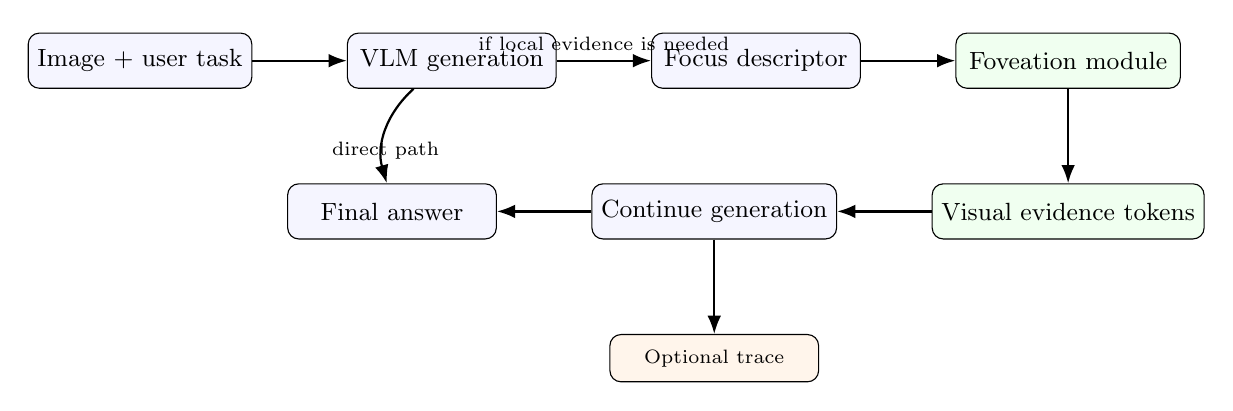
\begin{tikzpicture}[
  node distance=1.20cm,
  box/.style={draw, rounded corners, align=center, minimum height=0.70cm, minimum width=2.65cm, fill=blue!4, font=\small},
  tool/.style={draw, rounded corners, align=center, minimum height=0.70cm, minimum width=2.85cm, fill=green!6, font=\small},
  log/.style={draw, rounded corners, align=center, minimum height=0.60cm, minimum width=2.65cm, fill=orange!8, font=\scriptsize},
  arr/.style={-Latex, thick}
]
\node[box] (input) {Image + user task};
\node[box, right=of input] (gen) {VLM generation};
\node[box, right=of gen] (focus) {Focus descriptor};
\node[tool, right=of focus] (fov) {Foveation module};
\node[tool, below=of fov] (evidence) {Visual evidence tokens};
\node[box, left=of evidence] (resume) {Continue generation};
\node[box, left=of resume] (answer) {Final answer};
\node[log, below=of resume] (trace) {Optional trace};
\draw[arr] (input) -- (gen);
\draw[arr] (gen) -- node[above, font=\scriptsize]{if local evidence is needed} (focus);
\draw[arr] (focus) -- (fov);
\draw[arr] (fov) -- (evidence);
\draw[arr] (evidence) -- (resume);
\draw[arr] (resume) -- (answer);
\draw[arr] (gen) to[bend right=32] node[below, font=\scriptsize]{direct path} (answer);
\draw[arr] (resume) -- (trace);
\end{tikzpicture}
\caption{Runtime loop of the current \method{} tool. The model either answers directly or emits an inspectable focus request. The tool converts the request into target-conditioned visual evidence and resumes generation.}
\label{fig:runtime-loop}
\end{figure*}

\section{Current Tool Components}

\subsection{Focus-Capable Language Model}

The base VLM is trained to produce ordinary answers and, when useful, a bounded focus action. The focus action is part of generation rather than an external detector decision. This gives the model responsibility for deciding when its current evidence is insufficient. It also makes the request visible to downstream users, because the descriptor is natural language.

A well-formed focus action has three properties. It is \emph{specific}, naming the visual target rather than the whole image. It is \emph{grounded}, referring to visible regions, objects, text, or attributes. It is \emph{answer-relevant}, because the requested evidence should help resolve the user task. Descriptors that simply restate the question, ask for the entire image, or describe nonvisual reasoning are treated as low-quality actions.

\subsection{Visual Foveation Module}

The foveation module maps a descriptor-conditioned query and image visual features into a visual evidence sequence. The current implementation uses the descriptor hidden states as the conditioning signal. This is useful because the hidden states encode both the text of the descriptor and the model's local generation context. The image features provide the visual source from which the new evidence is produced.

The module is trained to satisfy two requirements. First, the evidence must be readable by the continuing VLM. Second, it must be target-specific: changing the descriptor or inserting mismatched evidence should reduce downstream performance. These requirements are important because a generic extra token block could improve formatting or act as a soft prompt without actually carrying the requested visual evidence.

\subsection{Runtime Controller}

The runtime controller implements the tool behavior around the model. It monitors generated tokens, detects a focus span, validates its boundaries, extracts descriptor hidden states, invokes the foveation module, inserts evidence tokens, and resumes generation. It also records an audit trace. A compact trace may contain the emitted descriptor, whether the direct path or re-focus path was used, evidence token shape, malformed-span flags, repeated-focus flags, and answer parsing status.

The controller also enforces practical limits. For example, deployment can set a maximum number of focus calls, reject malformed descriptors, suppress repeated requests for the same target, or fall back to direct answering when tool execution fails. These controls keep the tool usable in latency-sensitive and reliability-sensitive settings.

\section{Inference Procedure}

The current inference procedure is shown in Table~\ref{tab:inference}. The direct path and the re-focus path share the same initial image and task encoding. The difference is whether generation terminates with an answer or pauses for evidence insertion.

\begin{table}[t]
\centering
\small
\caption{Inference procedure}
\label{tab:inference}
\begin{tabular}{p{0.15\columnwidth}p{0.74\columnwidth}}
\toprule
Step & Operation \\
\midrule
1 & Encode the image and user task with the VLM. \\
2 & Generate until the model emits either an answer or a focus request. \\
3 & If an answer appears, return the answer through the direct path. \\
4 & If a focus request appears, parse the descriptor span and validate boundaries. \\
5 & Extract descriptor hidden states, excluding boundary tokens. \\
6 & Generate visual evidence tokens from image features conditioned on the descriptor states. \\
7 & Insert the evidence block into the active context. \\
8 & Resume generation and return the final answer, or allow another bounded focus step if enabled. \\
\bottomrule
\end{tabular}
\end{table}

This procedure supports a small number of repeated focus steps, but a single re-focus is often the preferred operating point. It captures most of the value of active visual inspection while keeping runtime cost predictable.

\section{Training Procedure}

Training is organized around two capabilities: producing useful visual evidence and learning when to use that evidence.

\subsection{Evidence Training}

The foveation module is trained on examples where an image and a focus descriptor determine a target visual detail. The model learns to generate evidence tokens that allow the downstream VLM to recover the requested information or answer a related question. The descriptor hidden states are used as the query, and image features are used as the visual source.

A central part of evidence training is control evaluation. The system compares correct evidence against no evidence, random evidence, evidence generated for the wrong target in the same image, and evidence generated from a different image. If correct evidence helps while mismatched evidence fails, the module is more likely to be carrying target-specific visual information rather than simply injecting helpful extra context.

\subsection{Trajectory Training}

The VLM is trained on mixed trajectories. Some examples require direct answering, and others require a focus request followed by evidence readout and answer generation. This teaches the model not only the syntax of the tool action, but also a routing policy. The desired behavior is conditional: use the tool when the question depends on missing local evidence, and avoid tool use when the answer is already visible enough.

The training target therefore includes four behaviors: valid focus-boundary generation, concise descriptor writing, continuation after evidence insertion, and direct answering without unnecessary tool use. These behaviors are evaluated separately because a model can learn the boundary format without learning good routing, or learn routing without reading the returned evidence effectively.

\section{Evaluation Snapshot}

The current evaluation supports the mechanism that target-conditioned visual evidence improves the model's ability to answer when local evidence is needed. Table~\ref{tab:evaluation} summarizes the available implementation snapshot. These numbers should be treated as current tool evidence rather than broad benchmark claims.

\begin{table*}[t]
\centering
\small
\caption{Current evaluation summary}
\label{tab:evaluation}
\begin{tabular}{p{0.20\linewidth}p{0.25\linewidth}p{0.45\linewidth}}
\toprule
Area & Observed result & Interpretation \\
\midrule
Evidence readability & Correct evidence reaches 100\% readout accuracy in the evaluated setting. & The generated visual evidence can be consumed by the model context. \\
Target specificity & Retrieval top-1 is 74.5\%, top-2 is 94.0\%, and MRR is 86.1\%. & The evidence is sensitive to the requested focus target. \\
Mismatched controls & Wrong-target and random-evidence controls degrade performance relative to correct evidence. & Gains are not explained only by adding extra tokens or using a special block format. \\
Boundary control & Focus-start accuracy reaches 1.0, with high focus-end and mean boundary scores. & The model learns a parseable tool-action format. \\
Controlled answering & Correct evidence reaches 87.50\% under forced tool use and 89.84\% under teacher-forced evidence insertion. & Correct visual evidence improves answer behavior under controlled insertion. \\
Free routing & Correct triggered cases reach 72.73\%; no-focus false triggering is 0 in the cited evaluation slice. & The model has learned a usable routing behavior, though calibration can still improve. \\
\bottomrule
\end{tabular}
\end{table*}

The most important result is the control pattern. Correct evidence performs better than no evidence, random evidence, and mismatched evidence. This indicates that the tool contributes information aligned with the focus request. The free-routing result is also important, but it should be interpreted separately: routing quality measures whether the model chooses the tool appropriately, while evidence quality measures whether the tool output is useful once invoked.

\section{Interface and Logging}

A practical deployment can expose a simple interface while keeping tensor-level details internal. Table~\ref{tab:interface} lists the recommended fields.

\begin{table}[t]
\centering
\small
\caption{Suggested interface fields}
\label{tab:interface}
\begin{tabular}{p{0.31\columnwidth}p{0.58\columnwidth}}
\toprule
Field & Description \\
\midrule
Input image & Original image or precomputed visual features. \\
User task & Natural-language question or instruction. \\
Maximum focus steps & Upper bound on re-focus calls per answer. \\
Final answer & The model response returned to the user. \\
Focus trace & Optional emitted focus descriptors. \\
Evidence metadata & Optional token count, shape, norm, or insertion status. \\
Routing status & Direct path, tool path, malformed span, repeated focus, or fallback. \\
Latency metrics & Time spent in generation, foveation, and continuation. \\
\bottomrule
\end{tabular}
\end{table}

For ordinary users, the focus descriptor is the most useful trace artifact because it explains what the model tried to inspect. For developers, evidence metadata and routing flags are useful for diagnosing malformed requests, repeated tool calls, weak descriptors, or cases where the tool was used but the answer remained wrong.

\section{Use Cases}

The tool is most appropriate for VLM applications where a model can benefit from a targeted second look without invoking a full specialist pipeline. Representative use cases include:

\begin{itemize}
  \item \textbf{Product and package QA}: reading small labels, checking expiration dates, identifying printed codes, and verifying local package attributes.
  \item \textbf{Technical troubleshooting}: inspecting connectors, switches, cables, indicator lights, assembly states, and localized damage.
  \item \textbf{Document-adjacent reasoning}: focusing on a specific field, table cell, handwritten note, stamp, or marginal annotation when full OCR is unnecessary or too costly.
  \item \textbf{Chart and dashboard understanding}: re-checking marks, legends, axis labels, small values, and local trend features.
  \item \textbf{Human-review workflows}: exposing a model's visual evidence request so that reviewers can understand why the answer depended on a particular region or attribute.
\end{itemize}

\section{Deployment Constraints}

The current tool requires more access than a black-box text-only API. A compatible runtime should provide generated hidden states for the focus descriptor span, image visual features or access to a local visual encoder, a trained foveation module, and a controller that can pause and resume generation around evidence insertion.

Latency depends on the number of focus calls and the evidence-token budget. In a production environment, the default configuration should use a small maximum number of focus steps, often one or two. Applications can also gate tool use with task type, confidence, descriptor quality, or latency budget.

Robustness requires fallback behavior. If the model emits malformed boundaries, an empty descriptor, a repeated descriptor, or a descriptor that is too broad, the controller should either reject the tool call or continue with a direct answer. Logging should distinguish these cases from ordinary wrong answers, because they indicate different failure modes.

\section{Limitations}

The current implementation has several limitations.

\begin{itemize}
  \item It depends on hidden-state and visual-feature access, so it is not directly portable to closed serving endpoints that expose only text responses.
  \item It improves targeted evidence acquisition, but it is not a complete replacement for OCR, detection, segmentation, or structured document processing.
  \item Free routing is useful but still calibratable; some deployments may prefer forced, policy-gated, or confidence-gated tool use.
  \item The current evaluation demonstrates the mechanism, but broader benchmark reporting requires task-standard evaluation settings and fixed reporting protocols.
  \item Multiple focus steps increase latency and can introduce repeated or low-value requests if not controlled.
\end{itemize}

\section{Conclusion}

\method{} adds a compact active-perception loop to vision-language model inference. The model can describe what it needs to inspect, the tool converts that descriptor into target-conditioned visual evidence, and generation continues with the new evidence available. The current implementation preserves a direct-answer path, supports bounded re-focus, provides an inspectable focus trace, and shows through controls that correct visual evidence is more useful than random or mismatched evidence. This makes the tool suitable for applications where local visual details matter and where answer behavior benefits from an explicit, debuggable visual re-inspection step.

\end{document}
